\chapter{លក្ខណៈកម្តៅនៃរូបធាតុ}
\begin{center}
	{\Large \kml\color{magenta}មេរៀនសង្ខេប}
\end{center}
\section{គំរូម៉ូលេគុលស៊ីនេទិចនៃឧស្ម័នបរិសុទ្ធ}
\quad យើងសិក្សាចលនាម៉ូលេគុលក្នុងធុងមួយ។ យើងបានសម្ពាធដែលសង្តត់លើផ្ទៃធុងគឺជាកម្លាំងទង្គិចរបស់ចលនាម៉ូលេគុល
\begin{align*}
\text{យើងបាន}\quad :&\quad P=\frac{F}{A}\quad \text{ដោយ}: \quad F=m\frac{\Delta \upsilon_{x}}{\Delta t}=\frac{m\times2\upsilon_{x}}{\dfrac{2L}{\upsilon_{x}}}=\frac{m\upsilon^{2}_{x}}{L}\\
\text{យើងបាន}\quad :&\quad P=\frac{m\upsilon^{2}_{x}}{AL}=\frac{m\upsilon^{2}_{x}}{V}\\
\text{តែ}\quad :&\quad \left(\upsilon^{2}\right)_{av}=\left(\upsilon^{2}_{x}\right)_{av}+\left(\upsilon^{2}_{y}\right)_{av}+\left(\upsilon^{2}_{z}\right)_{av}=3\left(\upsilon^{2}_{x}\right)_{av}\\\text{ដែល}\quad :&\quad \left(\upsilon=\upsilon_{x}=\upsilon_{y}=\upsilon_{z}=\text{ថេរ}\right)\\
\text{នាំឲ្យ}\quad :&\quad \left(\upsilon^2_{x}\right)_{av}=\frac{1}{3}\left(\upsilon^2\right)_{av}\\
\text{យើងបានសម្ពាធលើផ្ទៃខាងនីមួយៗ កំណត់ដោយៈ}\quad :&\quad P=\frac{1}{3}\times\frac{m}{V}\left(\upsilon^{2}\right)_{av}\quad \text{ឬ}\quad P=\frac{1}{3}\rho\left(\upsilon^{2}\right)_{av}\\
\text{ដែល}\quad :&\quad \rho =\frac{m}{V}\left(\text{ម៉ាសមាឌ}\right)\\
\text{ម្យ៉ាងទៀត}\quad :&\quad m=m_{0}N\\
\text{យើងបាន}\quad :&\quad P=\frac{1}{3}\times\frac{Nm_{0}}{V}\left(\upsilon^{2}\right)_{av}=\frac{2N}{3V}\times\frac{1}{2}m_{0}\left(\upsilon^2\right)_{av}\\
\text{ដូចនេះ}\quad :&\quad P=\frac{2}{3}\times\frac{N}{V}K_{av}
\end{align*}
\section{សមីការភាពនៃឧស្ម័ន}
\subsection{សមីការភាពនៃឧស្ម័នបរិសុទ្ធៈ} 
\begin{multicols}{2}
	តាមពិសោធន៍បង្ហាញថាៈ
	\begin{itemize}
		\item សម្ពាធសមាមាត្រនឹងសីតុណ្ហភាព: \quad $P\propto T$
		\item សម្ពាធសមាមាត្រនឹងចំនួនម៉ូលេគុល: \quad $P\propto N$
		\item សម្ពាធច្រាសសមាមាត្រនឹងមាឌ: \quad $P\propto\frac{1}{V}$
	\end{itemize}
	\begin{figure}[H]
		\centering
		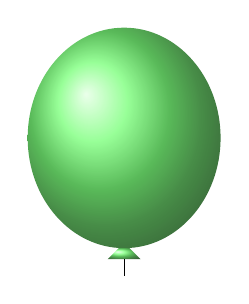
\begin{tikzpicture}[scale=.7]
		\begin{scope}
		\tikzstyle{balloon}=[ball color=green!60];    
		\shade[balloon, opacity=0.90] ellipse (1.75 and 2);
		\shade[balloon, opacity=0.90] (-.1,-2) -- (-.3,-2.2) -- (.3,-2.2) -- (.1,-2) -- cycle;
		\draw (0,-2.2) -- (0,-2.5);
		\end{scope}
		\end{tikzpicture}
		\caption{បាឡុងរាងស៊្វែផ្ទុកឧស្ម័ន}
	\end{figure}
\end{multicols}
\begin{align*}
\text{យើងបាន}\quad :& \quad P\propto \frac{NT}{V}\quad \text{ឬ}\quad P=k_{B}\frac{NT}{V}\quad \text{នោះ}\quad PV=Nk_{B}T\\\text{ដែល}\quad :&\quad k_{B}=1.38\times10^{-23}J/K\left(\text{ថេរបុលស្មាន់}\right)\\
\text{តែ}\quad :&\quad N=nN_{A}\quad \text{នោះ}\quad PV=nk_{B}N_{A}T\\
\text{តាង}\quad :&\quad R=k_{B}N_{A}\quad\text{ដែល}\quad N_{A}=6.02\times10^{23}\text{ម៉ូលេគុល}/mol\left(\text{ចំនួនអាវ៉ូកាដ្រូ}\right)\\
\text{ដូចនេះ}\quad :&\quad PV=Nk_{B}T=nRT=\frac{2}{3}NK_{av}
\end{align*}
\subsection{សមីការបម្រែបម្រួលភាពនៃឧស្ម័នបរិសុទ្ធៈ} បើឧស្ម័នប្រែប្រួលភាព ពីភាពដើម $1$ ទៅភាពស្រេច $2$ យើងបានៈ
\begin{itemize}
	\begin{multicols}{2}
		\item នៅភាពដើម $1$: $P_{1}V_{1}=nRT_{1}$ ឬ $\frac{P_{1}V_{1}}{T_{1}}=nR$
		\item នៅភាពស្រេច $2$: $P_{2}V_{2}=nRT_{2}$ ឬ $\frac{P_{2}V_{2}}{T_{2}}=nR$
	\end{multicols}
\end{itemize}
\begin{align*}
\text{យើងបាន}\quad :&\quad \frac{P_1V_1}{T_1}=\frac{P_2V_2}{T_2}=nR=\text{ថេរ}\\
\text{ច្បាប់ប៊យ-ម៉ារ្យ៉ូត}\quad :&\quad P_{1}V_{1}=P_{2}V_{2}\quad \left(\text{សីតុណ្ហភាពថេរ} T_{1}=T_{2}\right)\\
\text{ច្បាប់សាល}\quad :&\quad \frac{P_1}{T_1}=\frac{P_2}{T_2}\quad \left(\text{មាឌថេរ} V_{1}=V_{2}\right)\\
\text{ច្បាប់កេលុយសាក់}\quad :&\quad \frac{P_1V_1}{T_1}=\frac{P_2V_2}{T_2}\\
\end{align*}
\begin{formula}
	\begin{enumerate}[m]
		\item ម៉ាសមាឌ ឬដង់សុីតេមាឌនៃឧស្ម័នៈ $\rho=\frac{m}{V}=\frac{m_{0}N}{V}$\quad ដែល\quad $\rho$ គិតជា $\left(kg/m^3\right)$\\ $m$ ជាម៉ាសឧស្ម័ន គិតជា $\left(kg\right)$\\ $m_{0}$ ម៉ាសមូលេគុល គិតជា $\left(kg\right)$ 
		\\ $V$ មាឌឧស្ម័ន គិតជា $\left(m^3\right)$
		\item ចំនួនម៉ូលៈ $n=\frac{m}{M}=\frac{N}{N_{A}}=\frac{V}{V_{mol}}$\quad ដែល\quad $M$ ម៉ាសម៉ូលគិតជា $\left(kg/mol\right)$\\
		$N$ ចំនួនម៉ូលេគុលសរុប\\
		$V_{mol}$ ជាមាឌឧស្ម័នក្នុងមួយម៉ូល $\left(m^3/mol\right)$\\
		$V$ មាឌឧស្ម័ន $\left(m^3\right)$
		\item ចំនូនម៉ូលេគុលសរុបនៃឧស្ម័នៈ $N=\frac{m}{m_{0}}=nN_{A}=\frac{m}{M}\times N_{A}$ ដែល $n$ ចំនួនម៉ូល​ គិតជា $\left(mol\right)$
		\item មាឌម៉ូលនៃឧស្ម័នក្នុងលក្ខខ័ណ្ឌគំរូដែលមានសម្ពាធ $P_{0}=1atm$ និងសីតុណ្ហភាព $T=273K$ \\គឺៈ $V_{mol}=22.4\times10^{-3}m^3/mol$
		\item មាឌឧស្ម័នក្នុងមួយម៉ូល $V=V_{0}\left(1+\alpha T\right)$ ដែល $\alpha=\gamma=\frac{1}{273}$
	\end{enumerate}
\end{formula}
\newpage
\section{លំហាត់អនុវត្តន៍}
\begin{enumerate}
	\item ក្នុងធុងបិទជិតមួយមានឧស្ម័នអុីដ្រូសែន $\left(\ce{H2}\right)~0.2mol$ និងមានម៉ាសម៉ូល $2.0g/mol$។\\
	បើគេដឹងថា ចំនួនអាវ៉ូកាដ្រូ $N_{A}=6.022\times10^{23}$ម៉ូលេគុល$/mol$។
	\begin{enumerate}[k]
		\item គណនាចំនួនម៉ូលេគុលអុីដ្រូសែនក្នុងធុងនេះ។
		\item គណនាម៉ាសសរុបរបស់ឧស្ម័នអុីដ្រូសែន។
	\end{enumerate}
	\item ក្នុងធុងបិទជិតមួយមានឧស្ម័ន $0.25mol$ និងមានម៉ាសសរុប $7.0g$។\\
	បើគេដឹងថា ចំនួនអាវ៉ូកាដ្រូ $N_{A}=6.022\times10^{23}$ម៉ូលេគុល$/mol$។
	\begin{enumerate}[k]
		\item គណនាចំនួនម៉ូលេគុលសរុបរបស់ឧស្ម័នក្នុងធុងនេះ។
		\item តើឧស្ម័ននេះជាឧស្ម័នអ្វី?
	\end{enumerate}
	\item ក្នុងធុងបិទជិតមួយមានឧស្ម័នពេញ មានម៉ាសសរុប $64.0g$ និងមានចំនួនម៉ូលេគុលសរុបគឺ $12.044\times10^{23}$ម៉ូលេគុល។\\
	បើគេដឹងថា ចំនួនអាវ៉ូកាដ្រូ $N_{A}=6.022\times10^{23}$ម៉ូលេគុល$/mol$។
	\begin{enumerate}[k]
		\item គណនាចំនួនម៉ូលរបស់ឧស្ម័នក្នុងធុងនេះ។
		\item តើឧស្ម័ននេះជាឧស្ម័នអ្វី?
	\end{enumerate}
	\item ក្នុងធុងបិទជិតមួយមានផ្ទុក ឧស្ម័ន $\ce{H2}$ ពេញមានម៉ាសសរុប $1.0g$។ ដោយឧស្ម័ននេះមានម៉ាសម៉ូល $2.0g/mol$ និងចំនួនអាវ៉ូកាដ្រូ $N_{A}=6.022\times10^{23}$ម៉ូលេគុល$/mol$។
	\begin{enumerate}[k]
		\item គណនាចំនួនម៉ូលេគុលសរុបរបស់ឧស្ម័នក្នុងធុងនេះ។
		\item គណនាចំនួនម៉ូលរបស់ឧស្ម័ន $\ce{H2}$។
	\end{enumerate}
	\item ដបមួយផ្ទុកឧស្ម័នមានមាឌថេរក្រោមសម្ពាធថេរ $P_{0}=1.0atm$ នៅសីតុណ្ហភាព $17^\circ C$។ តើគេត្រូវកម្តៅឧស្ម័ននេះដល់សីតុណ្ហភាពប៉ុន្មានដើម្បីឧ្យសម្ពាធកើនឡើងដល់ $1.5atm$?
	\item គេបញ្ចូលអ៊ីដ្រូសែនទៅក្នុងបាឡុងមួយដែលមានមាឌ $100cm^{3}$ នៅសីតុណ្ហភាព $7^\circ$ ក្រោមសម្ពាធ $0.7atm$។ គណនាបំពង់អ៊ីដ្រូសែនដែលត្រូវប្រើដើម្បីបំប៉ោងបាឡុងនេះ បើបំពង់មួយមានអ៊ីដ្រូសែន $20\ell$ ក្រោមសម្ពាធ $150atm$ នៅសីតុណ្ហភាព $27^\circ C$ ដោយសន្មតថាឧស្ម័នក្នុងបំពង់ត្រូវបានបញ្ចូលទៅក្នុងបាឡុងទាំងអស់។
	\item គេយកបំពង់អុកស៊ីសែនមួយដែលមានចំណុះ $20\ell$ ក្រោមសម្ពាធ $P_{1}=200atm$ នៅសីតុណ្ហភាព $20^\circ C$ ទៅដាក់ក្នុងបាឡុងកៅស៊ូស្តើងមួយ។ គណនាមាឌបាឡុង បើឧស្ម័នក្នុងបឡុងមានសម្ពាធ $P_{2}=1atm$ និងសីតុណ្ហភាព $9^\circ C$។
	\item ប្រអប់មួយផ្តុកឧស្ម័នបរិសុទ្ធមានមាឌ $V=200cm^{3}$ មានសម្ពាធ $P=10atm$ នៅសីតុណ្ហភាព $27^\circ C$។ គណនាចំនួនម៉ូលគុលក្នុងប្រអប់បើថេរសកលនៃឧស្ម័នបរិសុទ្ធ $R=8.31J/mol\cdot K$។
	\item ម៉ាស៊ីនបូមខ្យល់មួយបូមខ្យល់បាន $66\ell$ ដាក់បញ្ចូលទៅក្នុងធុងដែលមានចំណុះ $6\ell$ ដោយសីតុណ្ហភាពឥតផ្លាស់ប្តូរស្តិតក្រោមសម្ពាធ $1atm$។ គណនាសម្ពាធចុងក្រោយរបស់ខ្យល់ក្នុងធុង។
	\item នៅសីតុណ្ហភាព $293K$ និងសម្ពាធ $5atm$ ឧស្ម័នមេតាន $1kmol$ មានម៉ាស $16.0kg$។ កណនាម៉ាសមាឌនៃមេតានក្នុងលក្ខខណ្ឌខាងលើ បើ $R=8.314J/mol\cdot K$។
	\item ធុងសាំងមួយមានចំណុះ $0.025m^{3}$ មានបរិមាណអាសូត $0.084kg$ កើនសម្ពាធបាន $3.17atm$ គណនាសីតុណ្ហភាពរបស់ឧស្ម័នអាសូត $\left(\ce{N2}\right)$ បើសម្ពាធបរិយាកាស $P_{atm}=1atm$ និងថេរសកលនៃឧស្ម័នបរិសុទ្ធ $R=8.31J/mol\cdot K$។
	\item នៅក្រោមសម្ពាធ $1atm$ នៅសីតុណ្ហភាព $15^\circ C$ ខ្យល់មានមាឌ $2\ell$។ គណនាសម្ពាធនៅសីតុណ្ហភាព $20^\circ C$ និងមានមាឌដដែល។
	\item គណនាចំនួនម៉ូលេគុលសរុបដែលមាននៅក្នុង $500g$ នៃខ្យល់។\\ បើគេដឹងថាក្នុងខ្យល់មានអុកសុីសែន​ $22\%$ និងមានអាសូត $78\%$ ជាម៉ាស។
	\item ក្នុងធុងបិទជិតមួយមានមាឌសរុប $16.62dm^3$ មានផ្ទុកឧស្ម័នបរិសុទ្ធពេញស្ថិតក្រោមសម្ពាធ $3\times10^{5}Pa$ និងមានសីតុណ្ហភាព $47^\circ C$។ គេឲ្យថេរឧស្ម័នបរិសុទ្ធ $R=8.31J/mol\cdot K$។ គណនាចំនួនម៉ូលនៃឧស្ម័នបរិសុទ្ធក្នុងធុងនោះ។
	\item បាឡុងពីរត្រូវបានតភ្ជាប់គ្នាដោយបំពង់មួយមានរ៉ូពីនេបិទជិត។ ដោយបាឡុងទី១ មានផ្ទុកឧស្ម័នដែលមានសម្ពាធ $5atm$ និងមានមាឌ $6L$ ចំណែកបាឡុងទី២នៅទទេមានមាឌ $4L$។\\ គេចាប់ផ្តើមបើករ៉ូពីនេ(បើគេដឹងថាបាឡុងនីមួយៗមានសីតុណ្ហភាពថេរ)។\\ គណនាសម្ពាធរបស់បាឡុងនីមួយៗ ក្រោយពេលគេបើករ៉ូពីនេ។
	\item បាឡុងពីរត្រូវបានតភ្ជាប់គ្នាដោយបំពង់មួយមានរ៉ូពីនេបិទជិត។ ដោយបាឡុងទី១ មានផ្ទុកឧស្ម័នដែលមានសម្ពាធ $6atm$ និងមានមាឌ $5L$ ចំណែកបាឡុងទី២ មានផ្ទុកឧស្ម័នដូចគ្នាដែលមានសម្ពាធ $4atm$ និងមានមាឌ $3L$។\\ គេចាប់ផ្តើមបើករ៉ូពីនេ(បើគេដឹងថាបាឡុងនីមួយៗមានសីតុណ្ហភាពថេរ)។\\ គណនាសម្ពាធរបស់បាឡុងនីមួយៗ ក្រោយពេលគេបើករ៉ូពីនេ។
	\item ឧស្ម័នអុកសុីសែនមួយម៉ូលមានសម្ពាធ $P_{1}$ នៅសីតុណ្ហភាព $27.0^\circ C$។
	\begin{enumerate}[k]
		\item បើឧស្ម័នត្រូវបានកម្តៅដោយរក្សាមាឌថេររហូតដល់សម្ពាធកើនឡើងបីដង ចូរគណនាសីតុណ្ហភាពនៃឧស្ម័ន។
		\item បើឧស្ម័នមានសម្ពាធ និងមាឌកើនឡើងពីរដង ចូរគណនាសីតុណ្ហភាពរបស់ឧស្ម័ន។
	\end{enumerate}
	\item នៅក្រោមផ្ទៃទឹកសមុទ្រជម្រៅ $25.0m$ មានម៉ាសមាឌ $\rho=1025kg/m^{3}$ មានសីតុណ្ហភាព $5^\circ C$។ ពពុះខ្យល់មួយមានមាឌ $1cm^{3}$ ផុសចេញមកលើផ្ទៃទឹកដែលមានសីតុណ្ហភាព $20^\circ C$។\\ គណនាមាឌរបស់ពពុះខ្យល់ពេលរៀបបែកចូលក្នុងខ្យល់។
	\item គេដាក់ទឹក $9.0g$ ទៅក្នុងធុងដែលមានចំណុះ $2.0L$ រួចដុតកម្តៅដល់សីតុណ្ហភាព $500^\circ C$។ គណនាសម្ពាធក្នុងធុង។
	\item សវនដ្ខានមួយមានវិមាត្រ $10.0m\times20.0m\times30.0m$។\\ គណនាចំនួនម៉ូលេគុលខ្យល់នៅក្នុងសវនដ្ខាននោះនៅកម្រិតសីតុណ្ហភាព $20.0^\circ C$ និងសម្ពាធ $101kPa$។
	\item \begin{enumerate}[k]
		\item បង្ហាញឲ្យឃើញថា ម៉ាសមាឌឧស្ម័នបរិសុទ្ធដែលមានមាឌ $V$ មានទំនាក់ទំនង់ $\rho =\frac{PM}{RT}$ ដែល $P$ ជាសម្ពាធឧស្ម័ន $M$ ជាម៉ាសម៉ូលឧស្ម័ន $T$ ជាសីតុណ្ហភាពឧស្ម័ន និង $R$ ជាថេរសកលនៃឧស្ម័ន។
		\item គណនាម៉ាសមាឌនៃឧស្ម័នអុកសុីសែននៅសម្ពាធធម្មតា និងសីតុណ្ហភាព $20.0^\circ C$។
	\end{enumerate}
	\item មាសមានម៉ាសម៉ូល $197g/mol$។
	\begin{enumerate}[k]
		\item គណនាចំនួនម៉ូលនៃអាតូមមាសក្នុងគម្រូមាសសុទ្ធ $2.50g$។
		\item គណនាចំនួនអាតូមដែលមានក្នុងគម្រូខាងលើ។
	\end{enumerate}
	\item គណនាៈ ចំនួនម៉ូល និងចំនួនម៉ូលេគុលក្នុង $1.00cm^{3}$ នៃឧស្ម័នបរិសុទ្ធនៅសម្ពាធ $100Pa$ និងសីតុណ្ហភាព $220K$។
\end{enumerate}
